\chapter{Tutorial}\label{tutorial}

\section{Introduction}\index{intro}
This tutorial has been developed by Brian Linkletter (http://www.brianlinkletter.com/mininet-wifi-software-defined-network-emulator-supports-wifi-networks). We thank Brian for his time and this helpful tutorial.

\section{First ideas}\index{First ideas}

In this post, I describe the unique functions available in the Mininet-WiFi network emulator and work through a few tutorials exploring its features.

\subsection{How to read this post}

In this post, I present the basic functionality of Mininet-WiFi by working through a series of tutorials, each of which works through Mininet-WiFi features, while building on the knowledge presented in the previous tutorial. I suggest new users work through each tutorial in order.

I do not attempt to cover every feature in Mininet-WiFi. Once you work through the tutorials in this post, you will be well equipped to discover all the features in Mininet-WiFi by working through the \texttt{Mininet-WiFi example scripts}- https://github.com/intrig-unicamp/mininet-wifi/tree/master/examples, and reading the \texttt{Mininet-WiFi wiki}\footnote{https://github.com/intrig-unicamp/mininet-wifi/wiki} and \texttt{mailing list}\footnote{https://groups.google.com/forum/\#!forum/mininet-wifi-discuss}.

I assume the reader is already familiar with the [Mininet network emulator](http://mininet.org/) so I cover only the new WiFi features added by Mininet-WiFi. If you are not familiar with Mininet, please read my \texttt{Mininet network simulator review}\footnote{http://www.brianlinkletter.com/mininet-test-drive/} before proceeding. I have also written \texttt{many other posts about Mininet}\footnote{http://www.brianlinkletter.com/tag/mininet/}.

I start by discussing the functionality that Mininet-WiFi adds to Mininet: Mobility functions and WiFi interfaces. Then I show how to install Mininet-WiFi and work through the tutorials listed below:

Tutorial \#1: One access point shows how to run the simplest Mininet-WiFi scenario, shows how to capture wireless traffic in a Mininet-Wifi network, and discusses the issues with OpenFlow and wireless LANs.

Tutorial \#2: Multiple access points shows how to create a more complex network topology so we can experiment with a very basic mobility scenario. It discusses more about OpenFlow and shows how the Mininet reference controller works in Mininet-WiFi.

Tutorial \#3: Python API and scripts shows how to create more complex network topologies using the Mininet-WiFi Python API to define node positions in space and other node attributes. It also discusses how to interact with nodes running in a scenario with the Mininet-WiFi CLI, the Mininet-WiFi Python interpreter, and by running commands in a node's shell.

Tutorial \#4: Mobility shows how to create a network mobility scenario in which stations move through space and may move in and out of range of access points. It also discusses the available functions that may be used to implement different mobility models using the Mininet-WiFi Python API.


\subsection{Mininet-WiFi compared to Mininet}

Mininet-WiFi is an extension of the Mininet software defined network emulator. The Mininet-WiFi developer did not modify any existing Mininet functionality, but added new functionality.

\subsection{Mininet-WiFi and Mobility}

Broadly defined, mobility in the context of data networking refers to the ability of a network to accommodate hosts moving from one part of the network to another. For example: a cell phone user may switch to a wifi access point when she walks into a coffee shop; or a laptop user may walk from her office in one part of a building to a meeting room in another part of the building and still being able to connect to the network via the nearest WiFi access point.

While the standard Mininet network emulator may be used to test mobility (In the Mininet examples folder, we find a \texttt{mobility.py} script that demonstrates methods that may be used to create a scenario where a host connected to one switch moves its connection to another switch), Mininet-WiFi offers more options to emulate complex scenarios where many hosts will be changing the switches to which they are connected. Mininet-WiFi adds new classes that simplify the programming work required by researchers to create Mobility scenarios.

Mininet-WiFi does not modify the reference SDN controller provided by standard Mininet so the reference controller cannot manage the mobility of users in the wireless network. Researchers must use a remote controller that supports the CAPWAP protocol (NOTE: I've not tried this and I do not know if it will work without modifications or additional programming), or manually add and delete flows in the access points and switches.

\subsection{802.11 Wireless LAN Emulation}

Mininet-wifi incorporates the Linux 802.11 SoftMAC\footnote{https://wireless.wiki.kernel.org/en/developers/documentation/glossary\#softmac} wireless drivers, the cfg80211\footnote{http://www.linuxwireless.org/en/developers/Documentation/cfg80211} wireless configuration interface and the mac80211\_hwsim\footnote{https://wireless.wiki.kernel.org/en/users/drivers/mac80211\_hwsim} wireless simulation drivers in its access points. 

The \texttt{mac80211\_hwsim} driver is a software simulator for Wi-Fi radios. It can be used to \texttt{create virtual wi-fi interfaces}\footnote{http://stackoverflow.com/questions/33091895/virtual-wifi-802-11-interface-similar-to-veth-on-linux} that use the \texttt{802.11 SoftMAC wireless LAN driver}\footnote{http://linuxwireless.org/en/developers/Documentation/mac80211/\_\_v49.html}. Using this tool, researchers may \texttt{emulate a Wi-Fi link between virtual machines}\footnote{https://w1.fi/cgit/hostap/plain/tests/hwsim/example-setup.txt} - some mac80211\_hwsim practical examples and supporting information are at the following links: \texttt{lab}\footnote{http://www2.cs.siu.edu/\~sharvey/code/cs441/cs441\_lab.pdf}, \texttt{thesis}\footnote{http://upcommons.upc.edu/bitstream/handle/2099.1/19202/memoria.pdf?sequence=4}, \texttt{hostapd}\footnote{https://nims11.wordpress.com/2012/04/27/hostapd-the-linux-way-to-create-virtual-wifi-access-point/}, \texttt{wpa-supplicant}\footnote{https://wiki.debian.org/WiFi/HowToUse\#wpa\_supplicant}, \texttt{docs-1}\footnote{https://www.kernel.org/doc/readme/Documentation-networking-mac80211\_hwsim-README}, and \texttt{docs-2}\footnote{https://github.com/penberg/linux-kvm/tree/master/Documentation/networking/mac80211\_hwsim))}. The 80211\_hwsim driver enables researchers to emulate the wifi protocol control messages passing between virtual wireless access points and virtual mobile stations in a network emulation scenario. By default, 80211\_hwsim simulates perfect conditions, which means there is no packet loss or corruption.

You can use Wireshark to \texttt{monitor wireless traffic}\footnote{http://sandilands.info/sgordon/capturing-wireless-lan-with-ubuntu-tcpdump-kismet} passing between the virtual wireless access point and the virtual mobile stations in the Mininet-wifi network scenarios. But, you will find it is difficult to capture wireless control traffic on standard WLAN interfaces like \texttt{ap1-wlan0} because the Linux kernel \texttt{strips wireless control messages and headers}\footnote{https://wiki.wireshark.org/Wi-Fi} before making traffic on these interfaces available to user processes like Wireshark. You will have to install additional tools and follow a complex procedure to \texttt{enable monitoring of WiFi traffic on the \texttt{ap1-wlan0} interface}\footnote{https://wiki.wireshark.org/CaptureSetup/WLAN\#Linux}. An easier method is available: look for the \texttt{hwsim0} interface on an access point, enable it, and monitor traffic on it. The \texttt{hwsim0} interface replays communications sent onto the access point's simulated wireless interface(s) such as \texttt{ap1-wlan0} without stripping any 802.11 headers or control traffic\footnote{from http://teampal.mc2lab.com/attachments/685/C2012-12.pdf}. We'll see this in the examples we work through, below.

\subsection{Mininet-WiFi display graph}

Since locations of nodes in space is an important aspect of WiFi networks, Mininet WiFi provides a graphical display (figure~\ref{fig:mngraph}) showing locations of WiFi nodes in a graph. The graph may be created by calling its method in the Mininet-WiFi Python API (see examples in the tutorials below).

\begin{figure}
    \centering
    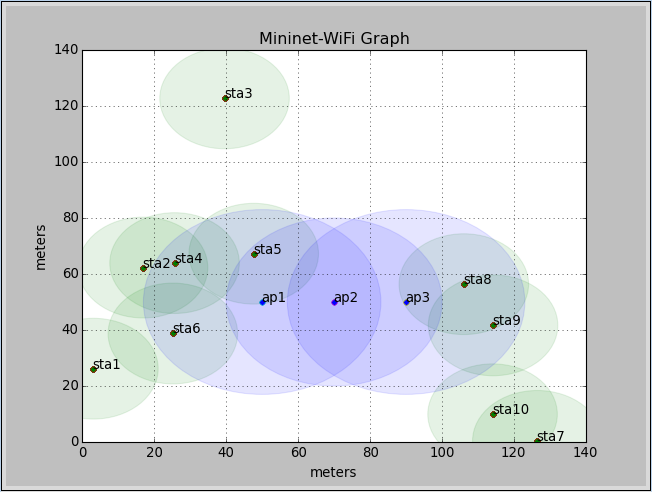
\includegraphics[width=0.7\textwidth]{Pictures/mn-wifi-graph-200}
    \caption{Mininet-WiFi Graph}
    \label{fig:mngraph}
\end{figure}

The graph will show wireless access points and stations, their positions in space and will display the affects of the range parameter for each node. The graph will not show any "wired" network elements such as standard Mininet hosts or switches, Ethernet connections between access points, hosts, or switches.

\subsection{Install Mininet-WiFi on a Virtual Machine}

First, we need to create a virtual machine that will run the Mininet-WiFi network emulator. In the example below, we will use the VirtualBox virtual machine manager because it is open-source and runs on Windows, Mac OS, and Linux.

\subsection{Set up a new Ubuntu Server VM}

Install Ubuntu Server in a new VM. Download an Ubuntu Server ISO image from the Ubuntu web site. See my post about \texttt{installing Debian Linux in a VM}\footnote{http://www.brianlinkletter.com/installing-debian-linux-in-a-virtualbox-virtual-machine/}. Follow the same steps to install Ubuntu.
\\
\\
In this example, we will name the VM \texttt{Mininet-WiFi}.

\subsection{Set up the Mininet-WiFi VM}

To ensure that the VM can display X applications such as Wireshark on your host computer's desktop, read through my post about \texttt{setting up the standard Mininet VM}\footnote{http://www.brianlinkletter.com/set-up-mininet/} and set up the host-only network adapter, the X windows server, and your SSH software.
\\
\\
Now you can connect to the VM via SSH with X Forwarding enabled. In the example below, my host computer is \texttt{t420} and the Mininet WiFi VM is named \texttt{wifi}.

\begin{minted}{bash}
t420:~$ ssh -X 192.168.52.101
wifi:~$
\end{minted}

\section{Mininet-WiFi Tutorial \#1: One access point}

The simplest network is the default topology, which consists of a wireless access point with two wireless stations. The access point is a switch connected to a controller. The stations are hosts.\\\\

\noindent This simple lab will allow us to demonstrate how to capture wireless control traffic and will demonstrate the way an OpenFlow-enabled access point handles WiFi traffic on the \texttt{wlan} interface.

\subsection{Capturing Wireless control traffic in Mininet-WiFi}

To view wireless control traffic we must first start Wireshark:

\begin{minted}{bash}
    wifi:~$ wireshark &
\end{minted}

\noindent Then, start Mininet-WiFi with the default network scenario using the command below:

\begin{minted}{bash}
    wifi:~$ sudo mn --wifi
\end{minted}

\noindent Next, enable the \texttt{hwsim0} interface. The \texttt{hwsim0} interface is the software interface created by Mininet-WiFi that copies all wireless traffic to all the virtual wireless interfaces in the network scenario. It is the easiest way to monitor the wireless packets in Mininet-WiFi.

\begin{minted}{bash}
    mininet-wifi> sh ifconfig hwsim0 up
\end{minted}

\noindent Now, in Wireshark (figure~\ref{fig:capture}, refresh the interfaces and then start capturing packets on the *hwsim0* interface. You should see wireless control traffic. Next, run a \texttt{ping} command:

\begin{minted}{bash}
    mininet-wifi> sta1 ping sta2
\end{minted}    

\begin{figure}
    \centering
    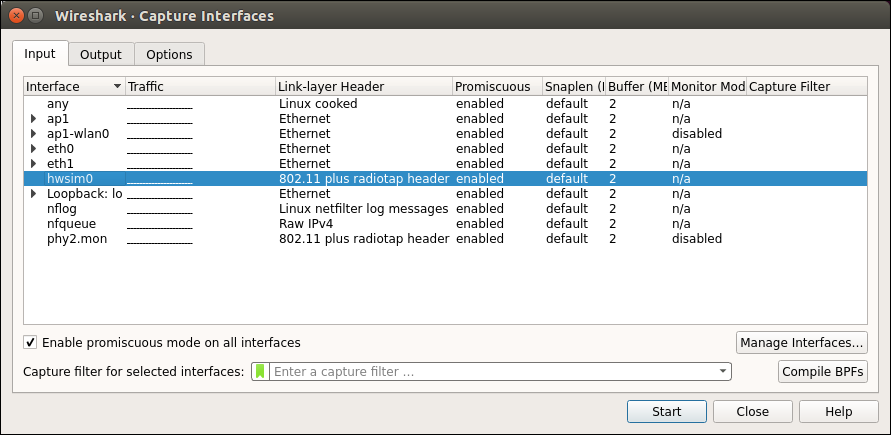
\includegraphics[width=0.7\textwidth]{Pictures/mn-wifi-008.png}
    \caption{Start capture on hwsim0 interface}
    \label{fig:capture}
\end{figure}

\noindent In Wireshark (figure~\ref{fig:traffic-wireshark}), see the wireless frames and the ICMP packets encapsulated in Wireless frames passing through the \texttt{hwsim0} interface. Stop the ping command by pressing \texttt{Ctrl-C}. In this default setup, any flows created in the access point (that's if they're created -- see below for more on this issue) will expire in 60 seconds.


\begin{figure}
    \centering
    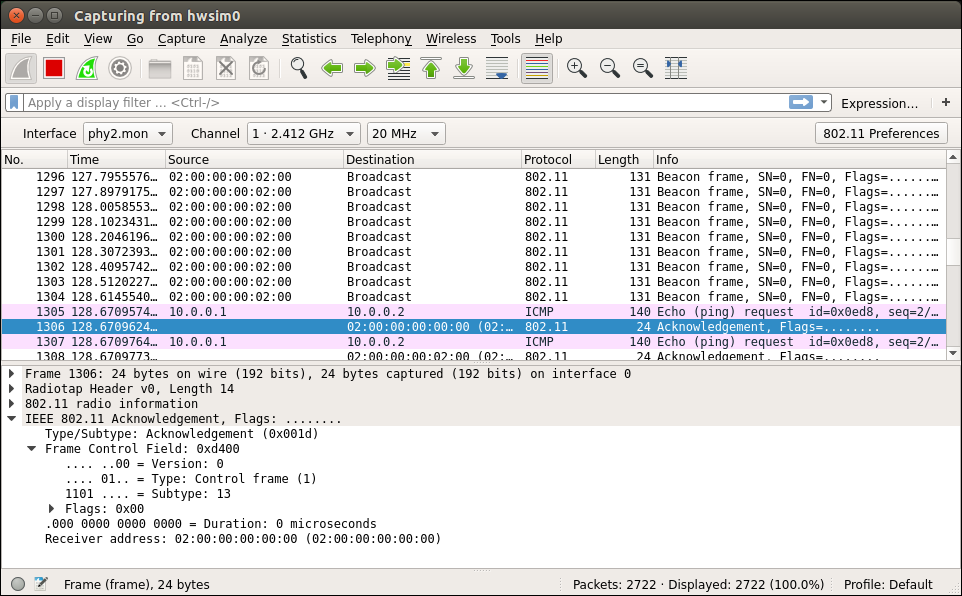
\includegraphics[width=0.7\textwidth]{Pictures/mn-wifi-010.png}
    \caption{Wireshark capturing WiFi control traffic}
    \label{fig:traffic-wireshark}
\end{figure}

\subsection{Wireless Access Points and OpenFlow}

In this simple scenario, the access point has only one interface, \texttt{ap1-wlan0}. By default, stations associated with an access point connect in \texttt{infrastructure mode} so wireless traffic between stations must pass through the access point. If the access point works similarly to a switch in standard Mininet, we expect to see OpenFlow messages exchanged between the access point and the controller whenever the access point sees traffic for which it does not already have flows established.

To view OpenFlow packets, stop the Wireshark capture and switch to the \texttt{loopback} interface. Start capturing again on the \texttt{loopback interface}. Use the \texttt{OpenFlow\_1.0} filter to view only OpenFlow messages.
\\
\\
\noindent Then, start some traffic running with the \texttt{ping} command and look at the OpenFlow messages captured in Wireshark.

\begin{minted}{bash}
    mininet-wifi> sta1 ping sta2
\end{minted}   

I was expecting that the first ICMP packet generated by the \texttt{ping} command should be flooded to the controller, and the controller would set up a flows on the access point so the two stations could exchange packets. Instead, I found that the two stations were able to exchange packets immediately and the access point did not flood the ICMP packets to the controller. Only an ARP packet, which is in a broadcast frame, gets flooded to the controller and is ignored (figure~\ref{fig:ofmsg}. \\

\begin{figure}
    \centering
    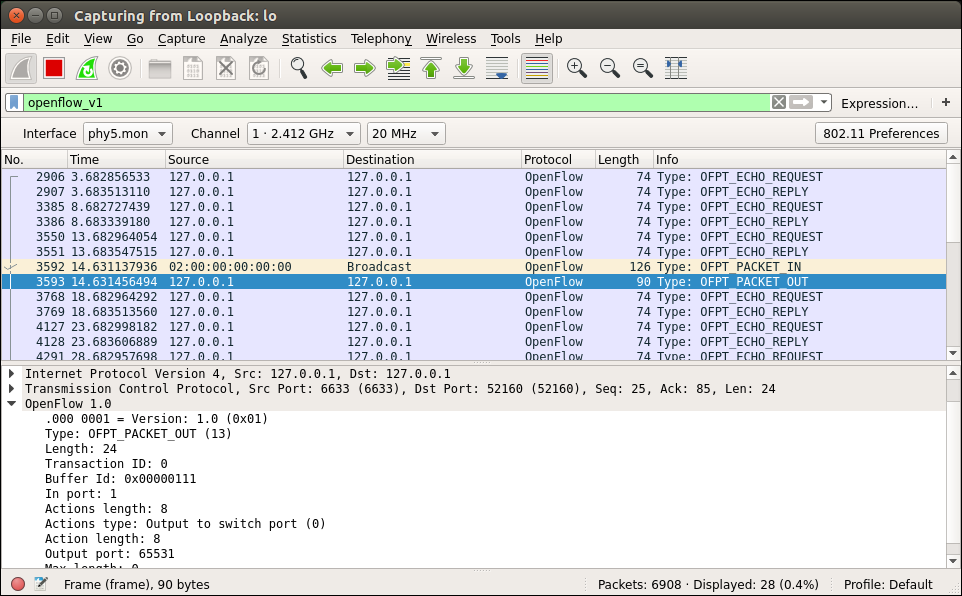
\includegraphics[width=0.7\textwidth]{Pictures/mn-wifi-20.png}
    \caption{No OpenFlow messages passing to the controller}
    \label{fig:ofmsg}
\end{figure}

\noindent Check to see if flows have been created in the access point:

\begin{minted}{bash}
    mininet-wifi> dpctl dump-flows
    *** ap1 ------------------------------------------
    NXST_FLOW reply (xid=0x4):
\end{minted}   

We see that no flows have been created on the access point. How do the two access points communicate with each other?

I do not know the answer but I have an idea. My research indicates that OpenFlow-enabled switches (using OpenFlow 1.0 or 1.3) will reject "hairpin connections", which are flows that cause traffic to be sent out the same port in which it was received. A wireless access point, by design, receives and sends packets on the same wireless interface. Stations connected to the same wireless access point would require a "hairpin connection" on the access point to communicate with each other. I surmise that, to handle this issue, Linux treats the WLAN interface in each access point like the radio network sta1-ap1-sta2 as if it is a "hub", where \texttt{ap1-wlan0} provides the "hub" functionality for data passing between sta1 and sta2. \texttt{ap1-wlan0} switches packets in the wireless domain and will not bring a packet into the "Ethernet switch" part of access point \texttt{ap1} unless it must be switched to another interface on \texttt{ap1} other than back out \texttt{ap1-wlan0}.

\subsection{Stop the tutorial}

Stop the Mininet \texttt{ping} command by pressing \texttt{Ctrl-C}. 

\noindent In the Wireshark window, stop capturing and quit Wireshark.

\noindent Stop Mininet-Wifi and clean up the system with the following commands:

\begin{minted}{bash}
    mininet-wifi> exit
    wifi:~$ sudo mn -c
\end{minted}
    
\section{Mininet-WiFi Tutorial \#2: Multiple access points}

When we create a network scenario with two or more wireless access points, we can show more of the functions available in Mininet-WiFi. 

In this tutorial, we will create a linear topology with three access points, where one station is connected to each access point. Remember, you need to already know \texttt{basic Mininet commands}\footnote{http://mininet.org/walkthrough/} to appreciate how we create topologies using the Mininet command line. 

Run Mininet-Wifi and create a linear topology with three access points:

\begin{minted}{bash}
    sudo mn --wifi --topo linear,3
\end{minted}
    
From the output of the command, we can see how the network is set up and which stations are associated with which access points.

\begin{minted}{bash}
*** Creating network
*** Adding controller
*** Adding hosts and stations:
sta1 sta2 sta3
*** Adding switches and access point(s):
ap1 ap2 ap3
*** Adding links and associating station(s):
(ap2, ap1) (ap3, ap2) (sta1, ap1) (sta2, ap2) (sta3, ap3)
*** Starting controller(s)
c0
*** Starting switches and access points
ap1 ap2 ap3 ...
*** Starting CLI:
mininet-wifi>
\end{minted}
    
We can also verify the configuration using the Mininet CLI commands \texttt{net} and \texttt{dump}. For example, we can run the \texttt{net} command to see the connections between nodes:

\begin{minted}{bash}
mininet-wifi> net
sta1 sta1-wlan0:None
sta2 sta2-wlan0:None
sta3 sta3-wlan0:None
ap1 lo:  ap1-eth1:ap2-eth1
ap2 lo:  ap2-eth1:ap1-eth1 ap2-eth2:ap3-eth1
ap3 lo:  ap3-eth1:ap2-eth2
c0
\end{minted}
    
From the \texttt{net} command above, we see that ap1, ap2, and ap3 are connected together in a linear fashion by Ethernet links. But, we do not see any information about to which access point each station is connect. This is because they are connected over a "radio" interface so we need to run the \texttt{iw} command at each station to observe to which access point each is associated.

To check which access points are "visible" to each station, use the \texttt{iw scan} command:

\begin{minted}{bash}
mininet-wifi> sta1 iw dev sta1-wlan0 scan | grep ssid
    SSID: ssid_ap1
    SSID: ssid_ap2
    SSID: ssid_ap3
\end{minted}

Verify the access point to which each station is currently connected with the \texttt{iw link} command. For example, to see the access point to which station \texttt{sta1} is connected, use the following command:

\begin{minted}{bash}
mininet-wifi> sta1 iw dev sta1-wlan0 link
    Connected to 02:00:00:00:03:00 (on sta1-wlan0)
            SSID: ssid_ap1
            freq: 2412
            RX: 1853238 bytes (33672 packets)
            TX: 7871 bytes (174 packets)
            signal: -30 dBm
            tx bitrate: 54.0 MBit/s
           
            bss flags:      short-slot-time
            dtim period:    2
            beacon int:     100
mininet-wifi>
\end{minted}
    

\subsection{A simple mobility scenario}

In this example, each station is connected to a different wireless access point. We can use the \texttt{iw} command to change which access point to which each station is connected. 

Note: The \texttt{iw} commands may be used in static scenarios like this but should not be used when Mininet-WiFi automatically assigns associations in more realistic mobility scenarios. We’ll discuss how Mininet-WiFi handles real mobility and how to use \texttt{iw} commands with Mininet-WiFi later in this post.

Let's decide we want \texttt{sta1}, which is currently associated with \texttt{ap1}, to change its association to \texttt{ap2}. Manually switch the \texttt{sta1} association from \texttt{ap1} (which is ssid\_ap1) to \texttt{ap2} (which is ssid\_ap2) using the following commands:

\begin{minted}{bash}
mininet-wifi> sta1 iw dev sta1-wlan0 disconnect
mininet-wifi> sta1 iw dev sta1-wlan0 connect ssid_ap2
\end{minted}

         
Verify the change with the \texttt{iw link} command:

\begin{minted}{bash}
mininet-wifi> sta1 iw dev sta1-wlan0 link
    Connected to 02:00:00:00:04:00 (on sta1-wlan0)
            SSID: ssid_ap2
            freq: 2412
            RX: 112 bytes (4 packets)
            TX: 103 bytes (2 packets)
            signal: -30 dBm
            tx bitrate: 1.0 MBit/s
    
            bss flags:      short-slot-time
            dtim period:    2
            beacon int:     100
mininet-wifi>
\end{minted}
    
We see that \texttt{sta1} is now associated with \texttt{ap2}. So we've demonstrated a basic way to make stations mobile, where they switch their association from one access point to another.

\subsection{OpenFlow flows in a mobility scenario}

Now let's see how the Mininet reference controller handles this simple mobility scenario. We need to get some traffic running from \texttt{sta1} to \texttt{sta3} in a way that allows us to access the Mininet-WiFi command line. We'll run the ping command in an \texttt{xterm} window on \texttt{sta3}.

First, check the IP addresses on \texttt{sta1} and \texttt{sta3} so we know which parameters to use in our test. The easiest way to see all IP addresses is to run the \texttt{dump} command:

\begin{minted}{bash}
mininet-wifi> dump
<Host sta1: sta1-wlan0:10.0.0.1 pid=7091>
<Host sta2: sta2-wlan0:10.0.0.2 pid=7094>
<Host sta3: sta3-wlan0:10.0.0.3 pid=7097>
<OVSSwitch ap1: lo:127.0.0.1,ap1-eth1:None pid=7106>
<OVSSwitch ap2: lo:127.0.0.1,ap2-eth1:None,ap2-eth2:None pid=7110>
<OVSSwitch ap3: lo:127.0.0.1,ap3-eth1:None pid=7114>
<Controller c0: 127.0.0.1:6633 pid=7080>
mininet-wifi> 
\end{minted}     

So we see that \texttt{sta1} has IP address 10.0.0.1 and \texttt{sta3} has IP address 10.0.0.3. Next, start an xterm window on \texttt{sta3}:

\begin{minted}{bash}
    mininet-wifi> xterm sta3
\end{minted}

This opens an xterm window (figure~\ref{fig:xterm} from \texttt{sta3}. 

\begin{figure}
    \centering
    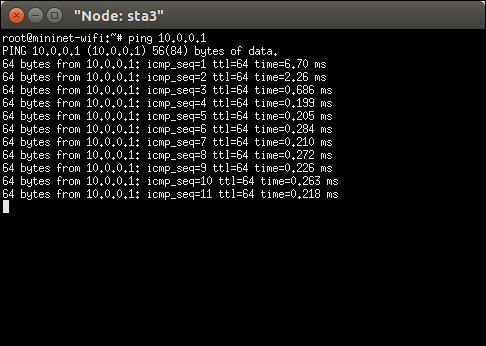
\includegraphics[width=0.7\textwidth]{Pictures/mn-wifi-102.png}
    \caption{xterm window on sta3}
    \label{fig:xterm}
\end{figure}


In that window, run the following command to send ICMP messages from \texttt{sta3} to \texttt{sta1}:     

\begin{minted}{bash}
    root@mininet-wifi:~# ping 10.0.0.1
\end{minted}

Since these packets will be forwarded by the associated access points out a port other then the port on which the packets were received, the access points will operate like normal OpenFlow-enabled switches. Each access point will forward the first ping packet it receives in each direction to the Mininet reference controller. The controller will set up flows on the access points to establish a connection between the stations \texttt{sta1} and \texttt{sta3}.

If we run Wireshark (figure~\ref{fig:wireshark} and enable packet capture on the \texttt{Loopback} interface, then filter using with \texttt{of} (for Ubuntu 14.04) or \texttt{openflow\_v1} (for Ubuntu 15.10 and later), we will see OpenFlow messages passing to and from the controller. Now, in the Mininet CLI, check the flows on each switch with the \texttt{dpctl dump-flows} command.

\begin{figure}
    \centering
    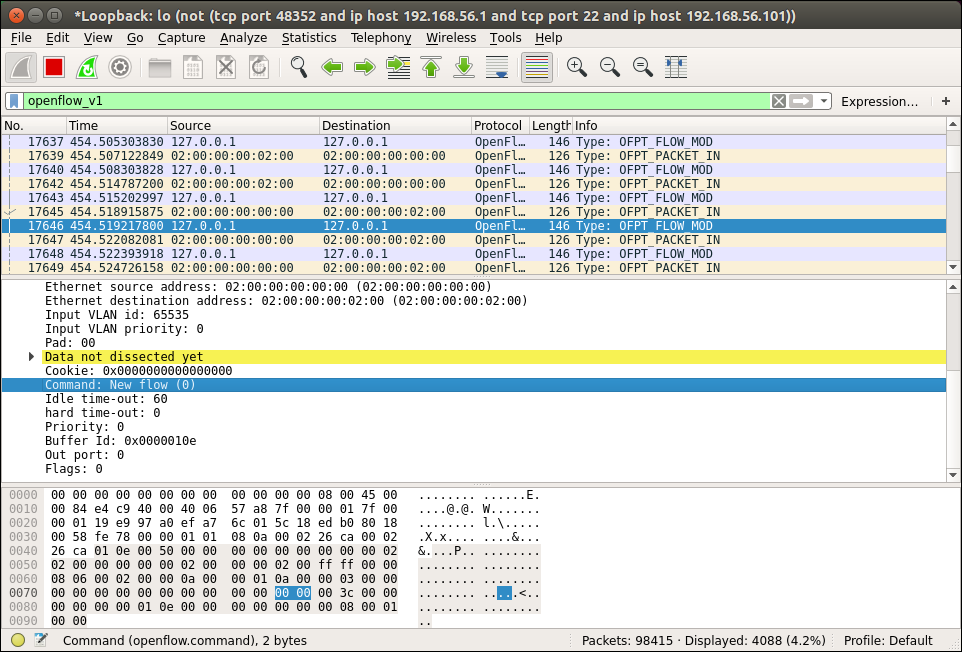
\includegraphics[width=0.8\textwidth]{Pictures/mn-wifi-121.png}
    \caption{Wireshark capturing OpenFlow messages}
    \label{fig:wireshark}
\end{figure}

\begin{minted}[breaklines]{bash}
mininet-wifi> dpctl dump-flows
    *** ap1 -----------------------------------------------
    NXST_FLOW reply (xid=0x4):
    *** ap2 -----------------------------------------------
    NXST_FLOW reply (xid=0x4):
    idle_timeout=60, idle_age=0, priority=65535,arp,in_port=2,vlan_tci=0x0000,dl_src=02:00:00:00:02:00, dl_dst=02:00:00:00:00:00,arp_spa=10.0.0.3,arp_tpa=10.0.0.1,arp_op=2 actions=output:3
     cookie=0x0, duration=1068.17s, table=0, n_packets=35, n_bytes=1470, idle_timeout=60, idle_age=0, priority=65535,arp,in_port=3,vlan_tci=0x0000,dl_src=02:00:00:00:00:00, dl_dst=02:00:00:00:02:00,arp_spa=10.0.0.1,arp_tpa=10.0.0.3,arp_op=1 actions=output:2
     cookie=0x0, duration=1073.174s, table=0, n_packets=1073, n_bytes=105154, idle_timeout=60, idle_age=0, priority=65535,icmp,in_port=3,vlan_tci=0x0000,dl_src=02:00:00:00:00:00, dl_dst=02:00:00:00:02:00,nw_src=10.0.0.1,nw_dst=10.0.0.3,nw_tos=0, icmp_type=0,icmp_code=0 actions=output:2
     cookie=0x0, duration=1073.175s, table=0, n_packets=1073, n_bytes=105154, idle_timeout=60, idle_age=0, priority=65535,icmp,in_port=2,vlan_tci=0x0000,dl_src=02:00:00:00:02:00, dl_dst=02:00:00:00:00:00,nw_src=10.0.0.3,nw_dst=10.0.0.1,nw_tos=0, icmp_type=8,icmp_code=0 actions=output:3
    *** ap3 -----------------------------------------------
    NXST_FLOW reply (xid=0x4):
     cookie=0x0, duration=1068.176s, table=0, n_packets=35, n_bytes=1470, idle_timeout=60, idle_age=0, priority=65535,arp,in_port=2,vlan_tci=0x0000,dl_src=02:00:00:00:02:00, dl_dst=02:00:00:00:00:00,arp_spa=10.0.0.3,arp_tpa=10.0.0.1,arp_op=2 actions=output:1
    idle_timeout=60, idle_age=0, priority=65535,arp,in_port=1,vlan_tci=0x0000,dl_src=02:00:00:00:00:00, dl_dst=02:00:00:00:02:00,arp_spa=10.0.0.1,arp_tpa=10.0.0.3,arp_op=1 actions=output:2
     cookie=0x0, duration=1073.182s, table=0, n_packets=1073, n_bytes=105154, idle_timeout=60, idle_age=0, priority=65535,icmp,in_port=1,vlan_tci=0x0000,dl_src=02:00:00:00:00:00, dl_dst=02:00:00:00:02:00,nw_src=10.0.0.1,nw_dst=10.0.0.3,nw_tos=0, icmp_type=0,icmp_code=0 actions=output:2
     cookie=0x0, duration=1073.185s, table=0, n_packets=1073, n_bytes=105154, idle_timeout=60, idle_age=0, priority=65535,icmp,in_port=2,vlan_tci=0x0000,dl_src=02:00:00:00:02:00, dl_dst=02:00:00:00:00:00,nw_src=10.0.0.3,nw_dst=10.0.0.1,nw_tos=0, icmp_type=8,icmp_code=0 actions=output:1
mininet-wifi>
\end{minted} 

We see flows set up on \texttt{ap2} and \texttt{ap3}, but not on \texttt{ap1}. This is because \texttt{sta1} is connected to \texttt{ap2} and \texttt{sta3} is connected to \texttt{ap3} so all traffic is passing through only \texttt{ap2} and \texttt{ap3}. What will happen if \texttt{sta1} moves back to \texttt{ap1}? Move \texttt{sta1} back to access point \texttt{ap1} with the following commands:

\begin{minted}{bash}
    mininet-wifi> sta1 iw dev sta1-wlan0 disconnect
    mininet-wifi> sta1 iw dev sta1-wlan0 connect ssid_ap1
\end{minted}

The \texttt{ping} command running on \texttt{sta3} stops working. We see no more pings completed.

In this case, access points \texttt{ap2} and \texttt{ap3} already have flows for ICMP messages coming from \texttt{sta3} so they just keep sending packets towards the \texttt{ap2-wlan0} interface to reach where they think \texttt{sta1} is connected. Since ping messages never get to \texttt{sta1} in its new location, the access point \texttt{ap1} never sees any ICMP traffic so does not request any flow updates from the controller.

Check the flow tables in the access points again: 

\begin{minted}[breaklines]{bash}
mininet-wifi> dpctl dump-flows
    *** ap1 -----------------------------------------------
    NXST_FLOW reply (xid=0x4):
     cookie=0x0, duration=40.959s, table=0, n_packets=1, n_bytes=42, idle_timeout=60, idle_age=40, priority=65535,arp,in_port=1,vlan_tci=0x0000,dl_src=02:00:00:00:02:00, dl_dst=02:00:00:00:00:00,arp_spa=10.0.0.3,arp_tpa=10.0.0.1,arp_op=1 actions=output:2
     cookie=0x0, duration=40.958s, table=0, n_packets=1, n_bytes=42, idle_timeout=60, idle_age=40, priority=65535,arp,in_port=2,vlan_tci=0x0000,dl_src=02:00:00:00:00:00, dl_dst=02:00:00:00:02:00,arp_spa=10.0.0.1,arp_tpa=10.0.0.3,arp_op=2 actions=output:1
    *** ap2 -----------------------------------------------
    NXST_FLOW reply (xid=0x4):
     cookie=0x0, duration=40.968s, table=0, n_packets=1, n_bytes=42, idle_timeout=60, idle_age=40, priority=65535,arp,in_port=2,vlan_tci=0x0000,dl_src=02:00:00:00:02:00, dl_dst=02:00:00:00:00:00,arp_spa=10.0.0.3,arp_tpa=10.0.0.1,arp_op=1 actions=output:1
     cookie=0x0, duration=40.964s, table=0, n_packets=1, n_bytes=42, idle_timeout=60, idle_age=40, priority=65535,arp,in_port=1,vlan_tci=0x0000,dl_src=02:00:00:00:00:00, dl_dst=02:00:00:00:02:00,arp_spa=10.0.0.1,arp_tpa=10.0.0.3,arp_op=2 actions=output:2
     cookie=0x0, duration=1214.279s, table=0, n_packets=1214, n_bytes=118972, idle_timeout=60, idle_age=0, priority=65535,icmp,in_port=2,vlan_tci=0x0000,dl_src=02:00:00:00:02:00, dl_dst=02:00:00:00:00:00,nw_src=10.0.0.3,nw_dst=10.0.0.1,nw_tos=0, icmp_type=8,icmp_code=0 actions=output:3
    *** ap3 -----------------------------------------------
    NXST_FLOW reply (xid=0x4):
     cookie=0x0, duration=40.978s, table=0, n_packets=1, n_bytes=42, idle_timeout=60, idle_age=40, priority=65535,arp,in_port=2,vlan_tci=0x0000,dl_src=02:00:00:00:02:00, dl_dst=02:00:00:00:00:00,arp_spa=10.0.0.3,arp_tpa=10.0.0.1,arp_op=1 actions=output:1
     cookie=0x0, duration=40.971s, table=0, n_packets=1, n_bytes=42, idle_timeout=60, idle_age=40, priority=65535,arp,in_port=1,vlan_tci=0x0000,dl_src=02:00:00:00:00:00, dl_dst=02:00:00:00:02:00,arp_spa=10.0.0.1,arp_tpa=10.0.0.3,arp_op=2 actions=output:2
     cookie=0x0, duration=1214.288s, table=0, n_packets=1214, n_bytes=118972, idle_timeout=60, idle_age=0, priority=65535,icmp,in_port=2,vlan_tci=0x0000,dl_src=02:00:00:00:02:00, dl_dst=02:00:00:00:00:00,nw_src=10.0.0.3,nw_dst=10.0.0.1,nw_tos=0, icmp_type=8,icmp_code=0 actions=output:1
mininet-wifi>
\end{minted}    

The controller sees some LLC messages from \texttt{sta1} but does recognize that \texttt{sta1} has moved to a new access point, so it does nothing. Since the controller does not modify any flows in the access points, none of the ICMP packets still being generated by \texttt{sta3} will reach \texttt{sta1} so it cannot reply. This situation will remain as long as the access points \texttt{ap2} and \texttt{ap3} continue to see ICMP packets from \texttt{sta3}, which keeps the old flow information alive in their flow tables.

One "brute force" way to resolve this situation is to delete the flows on the switches. In this simple example, it's easier to just delete all flows. Delete the flows in the access points using the command below: 

\begin{minted}{bash}
    mininet-wifi> dpctl del-flows
\end{minted}
    

Now the ping command running in the xterm window on \texttt{sta3} should show that pings are being completed again.

Once all flows were deleted, ICMP messages received by the access points do not match any existing flows so the access points communicate with the controller to set up new flows. If we dump the flows we see that the ICMP packets passing between \texttt{sta3} and \texttt{sta1} are now traversing across all three acces points.

\begin{minted}[breaklines]{bash}
mininet-wifi> dpctl dump-flows
    *** ap1 -----------------------------------------------
    NXST_FLOW reply (xid=0x4):
     cookie=0x0, duration=10.41s, table=0, n_packets=11, n_bytes=1078, idle_timeout=60, idle_age=0, priority=65535,icmp,in_port=2,vlan_tci=0x0000,dl_src=02:00:00:00:00:00, dl_dst=02:00:00:00:02:00,nw_src=10.0.0.1,nw_dst=10.0.0.3,nw_tos=0, icmp_type=0,icmp_code=0 actions=output:1
     cookie=0x0, duration=9.41s, table=0, n_packets=10, n_bytes=980, idle_timeout=60, idle_age=0, priority=65535,icmp,in_port=1,vlan_tci=0x0000,dl_src=02:00:00:00:02:00, dl_dst=02:00:00:00:00:00,nw_src=10.0.0.3,nw_dst=10.0.0.1,nw_tos=0, icmp_type=8,icmp_code=0 actions=output:2
    *** ap2 -----------------------------------------------
    NXST_FLOW reply (xid=0x4):
     cookie=0x0, duration=10.414s, table=0, n_packets=11, n_bytes=1078, idle_timeout=60, idle_age=0, priority=65535,icmp,in_port=1,vlan_tci=0x0000,dl_src=02:00:00:00:00:00, dl_dst=02:00:00:00:02:00,nw_src=10.0.0.1,nw_dst=10.0.0.3,nw_tos=0, icmp_type=0,icmp_code=0 actions=output:2
     cookie=0x0, duration=9.417s, table=0, n_packets=10, n_bytes=980, idle_timeout=60, idle_age=0, priority=65535,icmp,in_port=2,vlan_tci=0x0000,dl_src=02:00:00:00:02:00, dl_dst=02:00:00:00:00:00,nw_src=10.0.0.3,nw_dst=10.0.0.1,nw_tos=0, icmp_type=8,icmp_code=0 actions=output:1
    *** ap3 -----------------------------------------------
    NXST_FLOW reply (xid=0x4):
     cookie=0x0, duration=10.421s, table=0, n_packets=11, n_bytes=1078, idle_timeout=60, idle_age=0, priority=65535,icmp,in_port=1,vlan_tci=0x0000,dl_src=02:00:00:00:00:00, dl_dst=02:00:00:00:02:00,nw_src=10.0.0.1,nw_dst=10.0.0.3,nw_tos=0, icmp_type=0,icmp_code=0 actions=output:2
     cookie=0x0, duration=9.427s, table=0, n_packets=10, n_bytes=980, idle_timeout=60, idl_age=0, priority=65535,icmp,in_port=2,vlan_tci=0x0000,dl_src=02:00:00:00:02:00, dl_dst=02:00:00:00:00:00,nw_src=10.0.0.3,nw_dst=10.0.0.1,nw_tos=0, icmp_type=8,icmp_code=0 actions=output:1
mininet-wifi>
\end{minted}
    

We have shown how the Mininet reference controller works in Mininet-WiFi. The Mininet reference controller does not have the ability to detect when a station moves from one access point to another. When this happens, we must delete the existing flows so that new flows can be created. We will need to us a more advanced remote controller, such as OpenDaylight, to enable station mobility but that is a topic outside the scope of this post.

\subsection{Stop the tutorial}

Stop the Mininet \texttt{ping} command by pressing \texttt{Ctrl-C}. In the Wireshark window, stop capturing and quit Wireshark. Stop Mininet-Wifi and clean up the system with the following commands:

\begin{minted}{bash}
    mininet-wifi> exit
    wifi:~$ sudo mn -c
\end{minted}

\section{Mininet-WiFi Tutorial \#3: Python API and scripts}

Mininet provides a Python API so users can create simple Python scripts that will set up custom topologies. Mininet-WiFi extends this API to support a wireless environment.

When you use the normal Mininet \texttt{mn} command with the \texttt{--wifi} option to create Mininet-WiFi topologies, you do not have access to most of the extended functionality provided in Mininet-WiFi. To access features that allow you to emulate the behavior of nodes in a wireless LAN, you need to use the Mininet-Wifi extensions to the Mininet Python API.

\subsection{The Mininet-WiFi Python API}

The Mininet-WiFi developers added new classes to Mininet to support emulation of nodes in a wireless environment. Mininet-WiFi adds \texttt{addStation} and \texttt{addAccessPoint} methods, and a modified \texttt{addLink} method to define the wireless environment. 

If you are just beginning to write scripts for Mininet-WiFi, you can use the example scripts as a starting point. The Mininet-WiFi developers created example scripts that show how to use most of the features in Mininet-WiFi. In all of the tutorials I show below, I started with an example script and modified it. 

Mininet-Wifi example scripts are in the \texttt{~/mininet-wifi/examples} directory.

\subsection{Basic station and access point methods}

In a simple scenario, you may add a station and an access point with the following methods in a Mininet-WiFi Python script: \\

\noindent Add a new station named \texttt{sta1}, with all parameters set to default values:

\begin{minted}{bash}
    net.addStation( 'sta1' )
\end{minted}
    

\noindent Add a new access point named \texttt{ap1}, with SSID \texttt{ap1-ssid}, and all other parameters set to default values:
    
\begin{minted}{bash}
    net.addAccessPoint( 'ap1',  ssid='new_ssid' )
\end{minted}

\noindent Add a wireless association between station and access point, with default values for link attributes:

\begin{minted}{bash}
    net.addLink( ap1, sta1 )
\end{minted}
    
\noindent For more complex scenarios, more parameters are available for each method. You may specify the MAC address, IP address, location in three dimensional space, radio range, and more. For example, the following code defines an access point and a station, and creates an association (a wireless connection) between the two nodes and applies some traffic control parameters to the connection to make it more like a realistic radio environment, adding badwidth restrictions, an error rate, and a propagation delay:\\

\noindent Add a station and specify the wireless encryption method, the station MAC address, IP address, and position in virtual space:

\begin{minted}[breaklines]{bash}
    net.addStation( 'sta1', passwd='123456789a', encrypt='wpa2', mac='00:00:00:00:00:02', ip='10.0.0.2/8', position='50,30,0' ) 
\end{minted}
       
\noindent Add an access point and specify the wireless encryption method, SSID, wireless mode, channel, position, and radio range:

\begin{minted}[breaklines]{bash}
    net.addAccessPoint( 'ap1', passwd='123456789a', encrypt='wpa2', ssid= 'ap1-ssid', mode= 'g', channel= '1', position='30,30,0', range=30 )
\end{minted}    

To activate association control in a static network, you may use the *associationControl* method, which makes Mininet-WiFi automatically choose which access point a station will connect to based on the range between stations and access points. For example, use the following method to use the *strongest signal first* when determining connections between station and access points:

\begin{minted}{bash}
    net.associationControl( 'ssf' )
\end{minted}
    
\subsection{Classic Mininet API}

The Mininet WiFi Python API still supports the standard Mininet node types -- switches, hosts, and controllers. For example:\\

\noindent Add a host. Note that the station discussed above is a type of host nodem with a wireless interface instead of an Ehternet interface.

\begin{minted}{bash}
    net.addHost( 'h1' )
\end{minted}
    

\noindent Add a switch. Note that the access point discussed above is a type of switch that has one wireless interface (*wlan0*) and any number of Ethernet interfaces (up to the maximum supported by your installed version of Open vSwitch).

\begin{minted}{bash}
    net.addSwitch( 's1' )
\end{minted}
    

\noindent Add an Ethernet link between two nodes. Note that if you use *addLink* to connect two access points together (and are using the default Infrastructure mode), Mininet-WiFi creates an Ethernet link between them.

\begin{minted}{bash}
    net.addLink( s1, h1 )
\end{minted}
    
\noindent Add a controller:

\begin{minted}{bash}
    net.addController( 'c0' )
\end{minted}
        
\noindent Using the Python API, you may build a topology that includes hosts, switches, stations, access points, and multiple controllers.

\subsection{ Example }

In the example below, I created a Python program that will set up two stations connected to two access points, and set node positions and radio range so that we can see how these properties affect the emulated network. I used the Mininet-WiFi example script \texttt{2AccessPoints.py} as the base for the script shown below, then I added the position information to each node and enabled association control.

\lstinputlisting[language=Python]{codes/position-test.py}

I saved the file with the name \texttt{position-test.py} and made it executable. 

\subsection{Working at runtime}

Mininet-WiFi python scripts may be run from the command line by running the script directly, or by calling it as part of a Python command. The only difference is how the path is stated. For example:

\begin{minted}{bash}
    wifi:~/scripts $ sudo ./position-test.py
\end{minted}
or,
\begin{minted}{bash}
    wifi:~$ sudo python position-test.py
\end{minted}

The \texttt{position-test.py} script will set open the Mininet-WiFi graph window and show the locations of each wireless node in space (figure~\ref{fig:scriptrunning}, and the range attribute of each node.

\begin{figure}
    \centering
    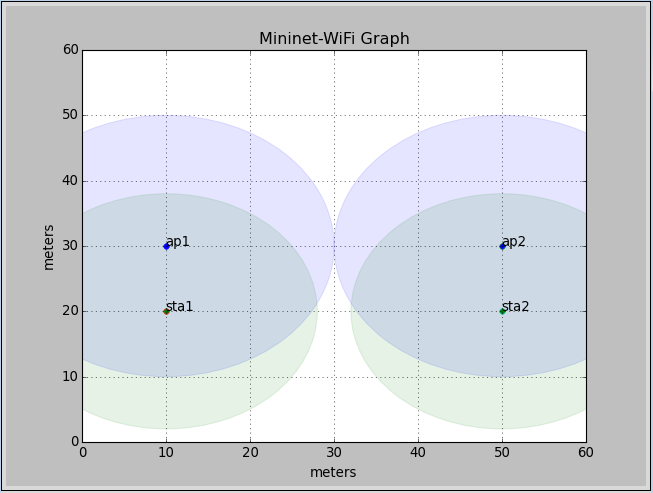
\includegraphics[width=0.7\textwidth]{Pictures/mn-wifi-graph-300.png}
    \caption{The position-test.py script running}
    \label{fig:scriptrunning}
\end{figure}

While the scenario is running, we can query information about the network from either the Mininet-WiFi command line or from the Python interpreter and we can log into running nodes to gather information or make configuration changes.

\subsection{Mininet-WiFi CLI}

The Python script \texttt{position-test.py} places nodes in specific positions. When the scenario is running, we can use the Mininet-WiFi command line interface (CLI) commands to can check the geometric relationship between nodes in space, and information about each node.

\subsection{Position}

The \texttt{position} CLI command outputs the location of a node in virtual space as measured by three values, one for each of the vertices X, Y, and Z.

Suppose we want to know the position of the access point \texttt{ap1} in the network scenario's virtual space. We may use the \texttt{position} CLI command to view a node's position:

\begin{minted}{bash}
    mininet-wifi> py ap1.params['position']
\end{minted}
   

We may also check the position of the station \texttt{sta2}:

\begin{minted}{bash}
    mininet-wifi> py sta.params['position']
\end{minted}
  
\subsection{Distance}

The \texttt{distance} CLI command tells us the distance between two nodes. For example, we may check how far apart access point \texttt{ap1} and station \texttt{sta2} are from each other using the \texttt{distance} CLI command:

\begin{minted}{bash}
    mininet-wifi> distance ap1 sta2        
    The distance between ap1 and sta2 is 41.23 meters
\end{minted}
       
\subsection{Mininet-WiFi Python runtime interpreter}

In addition to the CLI, Mininet-WiFi supports running Python code directly at the command line using the \texttt{py} command. Simple, Python functions may be called to get additional information about the network, or to make simple changes while the scenario is running.

\subsection{Getting network information}

The examples I show below are useful for gathering information about stations and access points.

To see the range of an access point or station, call the \texttt{range} function. Call it using the name of the node followed by the function as shown below for access point \texttt{ap1}:

\begin{minted}{bash}
    mininet-wifi> py ap1.params['range']
    20
\end{minted}
    
\noindent To see which station is associated with an access point (in this example \texttt{ap1}) call the \texttt{associatedStations} function:

\begin{minted}{bash}
    mininet-wifi> py ap1.associatedStations
    [<Host sta1: sta1-wlan0:10.0.0.1 pid=3845> ]
\end{minted}
   
\noindent To see which access point is associated with a station (in this example \texttt{sta1}) call the \texttt{associatedTo} key:

\begin{minted}{bash}
    mininet-wifi>py sta1.params['associatedTo']
    [<OVSSwitch ap1: lo:127.0.0.1,ap1-eth1:None pid=3862>]
\end{minted}
        

\noindent You may also query the received signal strength indicator (\texttt{rssi}), transmitted power (\texttt{txpower}), service set indicator (\texttt{ssid}), \texttt{channel}, and \texttt{frequency} of each wireless node using the Python interpreter.

\noindent As we can see, the output of Python functions is formatted as strings and numbers that may sometimes be hard to read. This is because these functions are built to support the program, not to be read by humans. However, if you which functions are available to be called at the Mininet-WiFi command line you will be able to get information you cannot get through the standard Mininet-WiFi CLI.

\subsection{Changing the network during runtime}

Mininet-WiFi provides Python functions that can be used during runtime to make changes to node positions and associations. These functions are useful when we have a static setup and want to make arbitrary changes on demand. This makes it possible to do testing or demonstrations with carefully controlled scenarios.

To change the access point to which a station is associated (provided the access point is within range):

\begin{minted}{bash}
    sta1.moveAssociationTo('sta1-wlan0', ap1) 
\end{minted}
    

\noindent To move a station or access point in space to another coordinate position:

\begin{minted}{bash}
    sta1.setPosition('40,20,40')
\end{minted}
    
\noindent To change the range of a station or access point:

\begin{minted}{bash}
    sta1.setRange(100)
\end{minted}    

The commands above will all impact which access points and which stations associate with each other. The behavior of the network will be different depending on whether association control is enabled or disabled in the \texttt{position-test.py} script.

\subsection{Running commands in nodes}

When running a scenario, users may make configuration changes on nodes to implement some additional functionality. This can be done from the Mininet-WiFi command line by sending commands to the node's command shell. Start the command with the name of the node followed by a space, then enter the command to run on that node.

\noindent For example, to see information about the WLAN interface on a station named \texttt{sta1}, run the command:

\begin{minted}{bash}
    mininet-wifi> sta1 iw dev sta1-wlan0 link
\end{minted}
    

\noindent Another way to run commands on nodes is to open an \texttt{xterm} window on that node and enter commands in the xterm window. For example, to open an xterm window on station *sta1*, run the command:

\begin{minted}{bash}
    mininet-wifi> xterm sta1
\end{minted}
    

\noindent Running commands on nodes is standard Mininet feature but it is also an advanced topic. See the \texttt{Mininet documentation}\footnote{https://github.com/mininet/mininet/wiki/Documentation} for more details. You can run simple commands such as \texttt{ping} or \texttt{iwconfig} but more advance commands may require you to mount \texttt{private directories}\footnote{https://github.com/mininet/mininet/wiki/Introduction-to-Mininet\#important-shared-filesystem} for configuration or log files.

\subsection{Mininet-WiFi and shell commands}

Mininet-WiFi manages the affect of range using code that calculates the ability of each node to connect with other nodes. However, Mininet-WiFi does not change the way networking works at the operating system level. So \texttt{iw} commands executed on nodes will override Mininet-WiFi and do not gather information generated by Mininet-WiFi about the network.

I suggest you do not rely on \texttt{iw} commands. For example, the \texttt{iw scan} command will still show that \texttt{sta1} can detect the SSIDs of all access points, even the access point \texttt{ap2} which should be out of range. The \texttt{iw link} command will show the same signal strength regardless of how far the station is from the access point, while the Mininet-WiFi *info* command will show the calculated signal strength based on the propagation model and distance between nodes.

For example, the \texttt{iw} command run on \texttt{sta1} shows received signal strength is -30 dBm. This never changes no matter how far the station is from the access point.


\begin{minted}{bash}
mininet-wifi> sta1 iw dev sta1-wlan0 link
Connected to 02:00:00:00:00:00 (on sta1-wlan0)
        SSID: ssid-ap1
        freq: 2412
        RX: 164628 bytes (2993 packets)
        TX: 775 bytes (10 packets)
        signal: -30 dBm
        tx bitrate: 6.0 MBit/s

        bss flags:      short-slot-time
        dtim period:    2
        beacon int:     100
\end{minted}
    

The \texttt{info} command shows Mininet-WiFi's calculated signal strength received by the station is -43.11 dBm. This value will change if you reposition the station.


\subsection{Stop the tutorial}

Stop Mininet-Wifi and clean up the system with the following commands:


\begin{minted}{bash}
    mininet-wifi> exit
    wifi:~$ sudo mn -c
\end{minted}

\section{Mininet-WiFi Tutorial \#4: Mobility}

The more interesting features provided by Mininet-WiFi support mobile stations moving around in virtual space. Mininet-Wifi provides new methods in its Python API, such as \texttt{startMobility} and \texttt{Mobility}, with which we may specify a wide variety of wireless LAN scenarios by controlling station movement, access point range, radio propagation models, and more.

In this tutorial, we will create a scenario where one station moves about in space, and where it changes which access point it connects to, based on which access point is the closest.

\subsection{Python API and mobility}

The Mininet-WiFi Python API adds new methods that allow the user to create stations that move around in virtual space when an emulation scenario is running.

To move a station in a straight line, use the \texttt{net.StartMobility} and \texttt{net.mobility} methods. See the example script \texttt{wifiMobilty.py}. For example, to move a station from one position to another over a period of 60 seconds, add the following lines to your script:

\begin{minted}{bash}
    net.startMobility( time=0 )
    net.mobility( 'sta1', 'start', time=1, position='10,20,0' )
    net.mobility( 'sta1', 'stop', time=59, position='30,50,0' )
    net.stopMobility( time=60 )
\end{minted}

    

Mininet-WiFi can also automatically move stations around based on predefined mobility models. See the example script \texttt{mobilityModel.py}. Available mobility models are: \texttt{RandomWalk}, \texttt{TruncatedLevyWalk}, \texttt{RandomDirection}, \texttt{RandomWayPoint}, \texttt{GaussMarkov}, \texttt{ReferencePoint}, and \texttt{TimeVariantCommunity}. For example, to move a station around in an area 60 meters by 60 meters with a minimum velocity of 0.1 meters per second and a maximum velocity of 0.2 meters per second, add the following line to your script:

\begin{minted}[breaklines]{bash}
    net.startMobility(time=0, model='RandomDirection', max_x=60, max_y=60, min_v=0.1, max_v=0.2)
\end{minted}    

Mininet-WiFi will automatically connect and disconnect stations to and from access points based on either calculated signal strength or load level. See the example script \texttt{wifiAssociationControl.py}. To use association control, add the \texttt{AC} parameter to the \texttt{net.startMobility} call. For example, to switch access points based on the “least loaded first” criteria, add the following line to your script:

\begin{minted}[breaklines]{bash}
    net.startMobility(time=0, model='RandomWayPoint', max_x=140, max_y=140, min_v=0.7, max_v=0.9, AC='llf')
\end{minted}

The valid values for the \texttt{AC} parameter are:

\begin{itemize}
\item llf (Least-Loaded-First)
\item ssf (Strongest-Signal-First)\\
\end{itemize}

When creating a scenario where stations will be mobile, we may set the range of the access points. In an example where we use “strongest signal first” as the Association Control method, the range of each access point will determine where handoffs occur between access points and which stations may connect to which access points. If you do not define the range, Mininet-WiFi assigns a default value. 

Mininet-WiFi supports more methods than mentioned above. See the example scripts (mentioned further below) for examples of using other methods.


\subsection{Moving a station in virtual space}

A simple way to demonstrate how Mininet-WiFi implements scenarios with mobile stations that hand off between access points is to create a script that moves one station across a path that passes by three access points.

The example below will create three access points -- \texttt{ap1}, \texttt{ap2}, and \texttt{ap3} -- arranged in a line at differing distances from each other. It also creates a host \texttt{h1} to serve as a test server and a mobile station \texttt{sta1} and moves \texttt{sta1} across space past all three access points.

\lstinputlisting[language=Python]{codes/line.py}

Save the script and call in \texttt{line.py}. Make it executable, then run the command:

\begin{minted}[breaklines]{bash}
    wifi:~$ sudo ./line.py
\end{minted} 

The Mininet-Wifi graph will appear (figure~\ref{fig:linescript}), showing the station and the access points. 

\begin{figure}[!b]
    \centering
    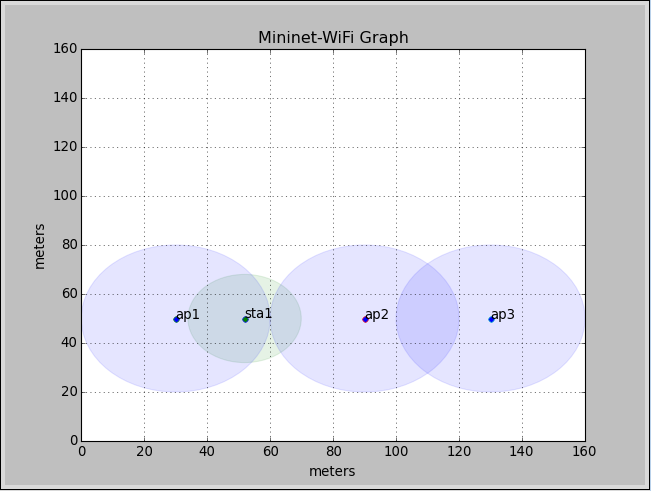
\includegraphics[width=0.7\textwidth]{Pictures/mn-wifi-graph-100}
    \caption{The line.py script running}
    \label{fig:linescript}
\end{figure}

The station \texttt{sta1} will sit still for 20 seconds, and then start to move across the graph from left to right for 60 seconds until it gets to the far side of the graph. The host \texttt{h1} and the virtual Ethernet connections between \texttt{h1}, \texttt{ap1} and between the three access points are not visible.

\subsection{Re-starting the scenario}

This simple scenario has a discreet start and stop time so, if you wish to run it again, you need to quit Mininet-WiFi, and start the script again. 

For example, suppose the scenario is at its end, where the station is now at the far right of the graph window. To stop and start it again, enter the following commands:

\begin{minted}{bash}
    mininet-wifi> exit
    wifi:~$ sudo mn -c
    wifi:~$ sudo ./line.py
\end{minted}    

\subsection{More Python functions}

When running a scenario with the mobility methods in the Python API, we have access to more information from Mininet-WiFi's Python functions. To see all access points that are within range of a station such as \texttt{sta1} at any time while the scenario is running, call the \texttt{apsInRange} function:

\begin{minted}{bash}
    mininet-wifi> py sta1.params['apsInRange']
    [<OVSSwitch ap1: lo:127.0.0.1,ap1-eth1:None pid=3862>]
\end{minted}
    
\subsection{Test with iperf}

To see how the system responds to traffic, run some data between host \texttt{h1} and station \texttt{sta1} when the scenario is started.\\

\noindent We have seen in previous examples how to use the \texttt{ping} program to create traffic. In this example, we will use the \texttt{iperf} program. First, start the \texttt{line.py} script again. Then start an iperf server on the station

\begin{minted}{bash}
    mininet-wifi> sta1 iperf --server 
\end{minted}
    

\noindent Then open an xterm window on the host \texttt{h1}. 

\begin{minted}{bash}
    mininet-wifi> xterm h1
\end{minted}
    

\noindent From the xterm window, we will start the iperf client command and create a stream of data between \texttt{h1} and \texttt{sta1}. On the \texttt{h1} xterm, run the command:

\begin{minted}{bash}
    iperf --client 10.0.0.2 --time 60 --interval 2 
\end{minted}

\noindent Watch the iperf output as the station moves through the graph. When it passes from one access point to the next, the traffic will stop. To get the traffic running again, clear the flow tables in the access points. In the Mininet-WiFi CLI, run the command shown below:

\begin{minted}{bash}
    mininet-wifi> dpctl del-flows
\end{minted}
    

\noindent Traffic should start running again. As stated in Tutorial \#2 above, we must clear flows after a hand off because the Mininet reference controller cannot respond correctly in a mobility scenario. The topic of configuring a remote controller to support a mobility scenario is outside the scope of this post. Clear the flows every time the station switches to the next access point.

\subsection{Stop the tutorial}

Stop Mininet-Wifi and clean up the system with the following commands:

\begin{minted}{bash}
    mininet-wifi> exit
    wifi:~$ sudo mn -c
\end{minted}

\section{Mininet-WiFi Tutorial \#5: VANETs (Veicular Ad Hoc Networks)}

\subsection{Python API}
The Mininet-WiFi python API add a new node that allow the user to create cars that move around in virtual space when an emulation scenario is running. The function addCar() defines this new node and you can see an example in the file vanet.py into /examples.

\subsection{Node Car Architecture}

The architecture of the node \texttt{car} is depicted in \autoref{fig:cararch}. In order to allow OpenFlow controllers to control simple nodes, like a car, it was necessary to create an architecture with a switch. Thus, every packet that comes from VehicleX needs to pass-trough VehicleXSW if the destination is a node in the wireless mesh network (like a Vehicle-to-Vehicle communication). The communication between cars and RSUs (Vehicle-to-Infrastructure), in turn, is done directly between VehicleX and the RSU. 

\begin{figure}[!t]
\centering
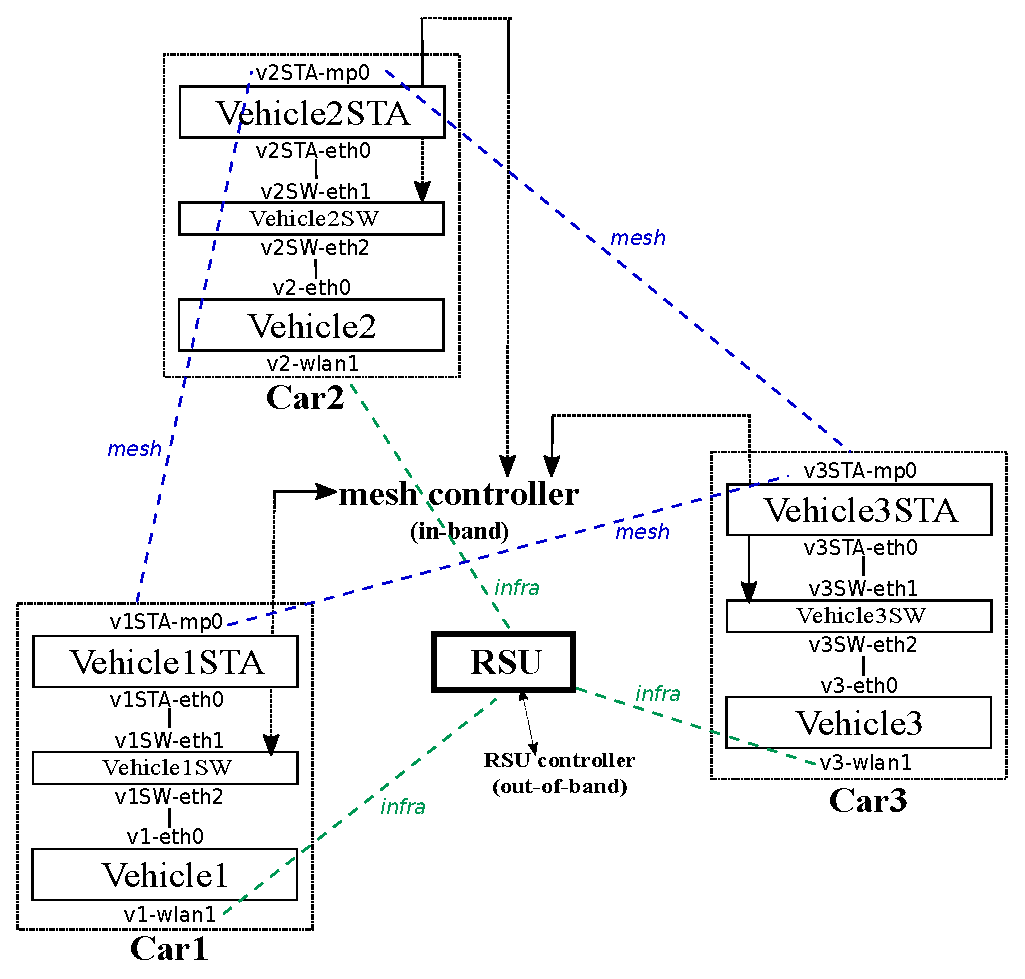
\includegraphics[width=0.6\textwidth]{Pictures/vanet.eps}
\caption{Node Car Architecture}
\label{fig:cararch}
\end{figure}

\begin{figure}[!b]
\centering
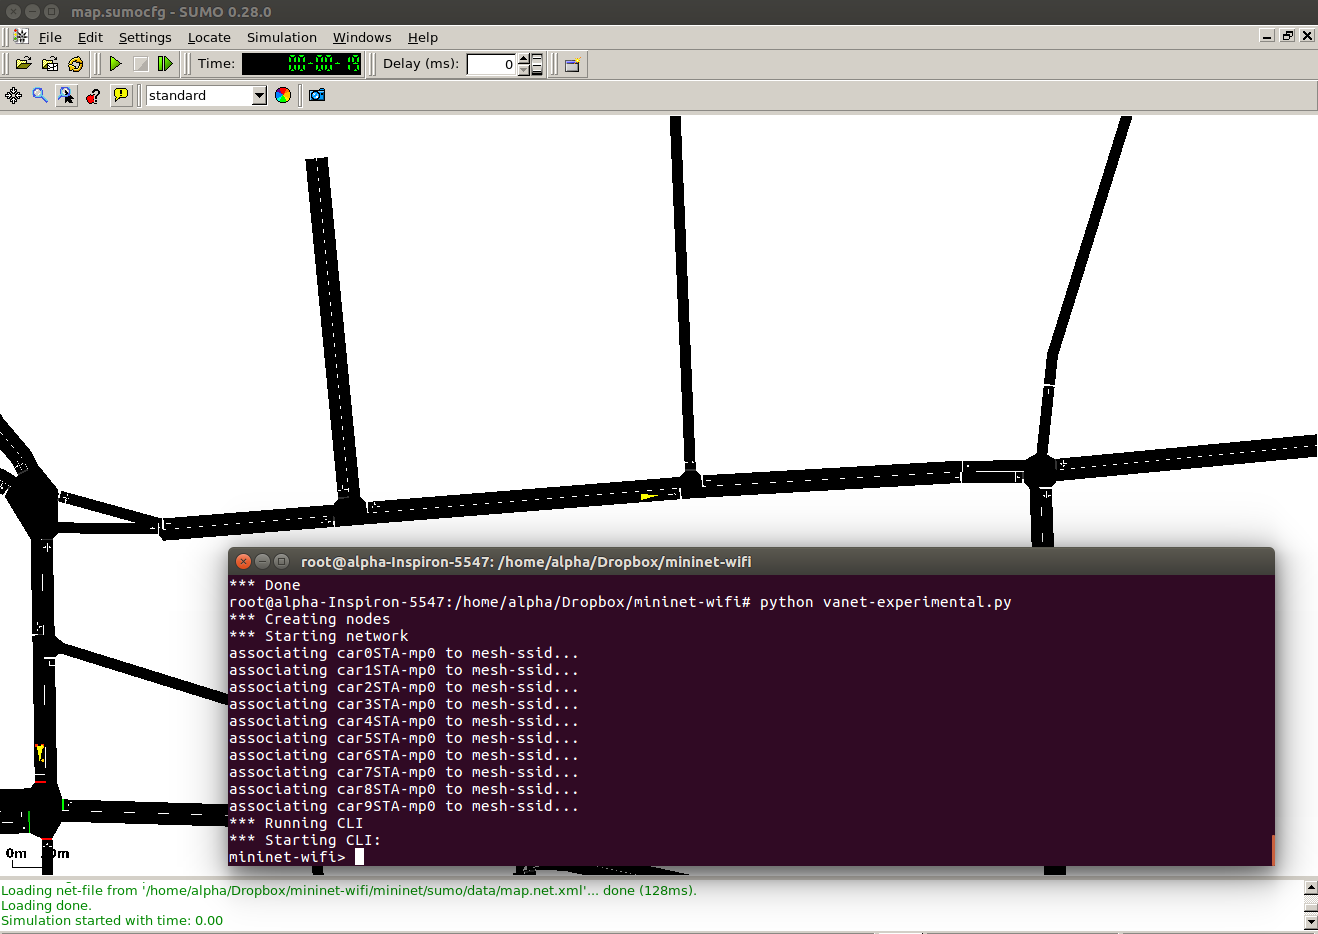
\includegraphics[width=0.6\textwidth]{Pictures/sumo.png}
\caption{Integration with SUMO}
\label{fig:sumo}
\end{figure}

\subsection{Integration with SUMO (Simulation of Urban Mobility)}
    
Mininet-WiFi already has some integration with SUMO. An example can be found in /examples/sumo-experimental.py.
    
\section{Mininet-WiFi example scripts}

The Mininet-WiFi developers created many example scripts that show examples of most of the API extensions they added to Mininet. They placed these example scripts in the folder \texttt{mininet-wifi/examples/}. Try running these scripts to see what they do and look at the code to understand how each feature is implemented using the Python API. Some interesting Mininet-WiFi example scripts are:

\texttt{adhoc} shows how to set up experiments with  adhoc mode, where stations connect to each other without passing through an access point.
\texttt{simplewifitopology} show the Python code that create the same topology as the default topology created my the \texttt{mn --wifi} command (two stations and one access point).
\texttt{position.py} shows how to create a network where stations and access points are places in specific locations in virtual space.
\texttt{mobility} and \texttt{mobilityModel} show how to move stations and how mobility models can be incorporated into scripts.
\texttt{wifiAssociationControl} shows how the different values of the AC parameter affect station handoffs to access points.
\texttt{wifimesh.py} shows how to set up a mesh network of stations.
\texttt{handover.py} shows how to create a simple mobility scenario where a station moves past two access points, causing the station to hand off from one to the other. 
\texttt{multipleWlan.py} shows how to create a station with more than one wireless LAN interface.
\texttt{propagationModel.py} shows how to use propagation models that impact how stations and access points can communicate with each other over distance.
\texttt{authentication.py} shows how to set up WiFi encryption and passwords on access points and stations.

\section{Conclusion}

The tutorials presented above work demonstrate many of the unique functions offered by Mininet-Wifi. Each tutorial revealed more functionality and we stopped at the point where we were able to emulate mobility scenario featuring a WiFi station moving in a straight line past several wireless access points. 

To learn more about Mininet-WiFi, go to the \texttt{Mininet-WiFi wiki}\footnote{https://github.com/intrig-unicamp/mininet-wifi/wiki} page. Also, read through posts on the \texttt{Mininet-WiFi mailing list}\footnote{https://groups.google.com/forum/\#!forum/mininet-wifi-discuss}, which is very active and is a useful source of more information about Mininet-WiFi. I am looking for an OpenFlow controller that will support WiFi switches using OpenFlow 1.3, which is the version of OpenFlow supported by Mininet and Mininet-WiFi. If you know of any, please add a comment to this post.

\begin{remark}
Thank you Brian Linkletter for this helpful tutorial.
\end{remark}